%===============================================================================
% $Id: ifacconf.tex 19 2011-10-27 09:32:13Z jpuente $  
% Template for IFAC meeting papers
% Copyright (c) 2007-2008 International Federation of Automatic Control
%===============================================================================
\documentclass[a4paper]{ifacconf}

\usepackage{graphicx,amsmath,url}      % include this line if your document contains figures
\usepackage[round]{natbib}             % required for bibliography
%===============================================================================


% ===============================================================
% Choose the language of the manuscript.
% If in English, choose 
% \def\portugues{0} 
%
% If in Portuguese or Spanish, choose
% \def\portugues{1} 
%
% Note that, if you are writing in Spanish, you need additional 
% adjusts in some parts of the text, which have been put in Portuguese only.
\def\portugues{1} 
% ===============================================================

% If the above line is commented, it is assumed manuscript in English:
\ifx\portugues\undefined
\def\portugues{0}
\fi


\if\portugues0
   \usepackage[english]{babel}
  \else
   \usepackage[spanish,brazil,english]{babel}
\fi

  

\usepackage[T1]{fontenc}
%\usepackage{inputenc}

\usepackage[utf8]{inputenc}

\usepackage{ae}


\if\portugues1
% =====================================================================
% =====================================================================
% If the manuscript is in Spanish, please change the texts adequatelly.
% You may also add other definitions in this part.
 \newtheorem{teorema}[thm]{{\em Teorema}}{ }
 \newtheorem{lema}[thm]{{\em Lema}}{ }
 \newtheorem{corolario}[thm]{{\em Corolário}}{ }
 \newenvironment{prova}{{\bf Prova.}}{ }
% ===============================================================
\fi

\begin{document}
	
	
\if\portugues1

% =====================================================================
% =====================================================================
% USE THIS PART IF THE TEXT IS IN PORTUGUES OR SPANISH
% =====================================================================
% If the manuscript is in Spanish, please change the texts adequately.
% =====================================================================
% 
\selectlanguage{brazil}
	
\begin{frontmatter}

\title{Estilo para Artigos em Português das Conferências da SBA --- Adaptado do  IFAC\thanksref{footnoteinfo}} 
% Title, preferably not more than 10 words.

\thanks[footnoteinfo]{Reconhecimento do suporte financeiro deve vir nesta nota de rodapé.}


\author[First]{Primeiro A. Autor} 
\author[Second]{Segundo B. Autor} 
\author[Third]{Terceiro C. Autor}

\address[First]{Faculdade de Engenharia Elétrica, Universidade do Triângulo, MG, (e-mail: autor1@faceg@univt.br).}
\address[Second]{Faculdade de Engenharia de Controle \& Automação, Universidade do Futuro, RJ (e-mail: autor2@feca.unifutu.rj)}
\address[Third]{Electrical Engineering Department, 
   Seoul National University, Seoul, Korea, (e-mail: author3@snu.ac.kr)}


\selectlanguage{english}
\renewcommand{\abstractname}{{\bf Abstract:~}}
\begin{abstract}                % Abstract of not more than 250 words.
These instructions give you guidelines for preparing papers for the Sociedade Brasileira de Automática (SBA) technical meetings using the IFAC style. Please use this document as a template to prepare your manuscript in portuguese. For submission guidelines, follow instructions on paper submission system as well as the event website.

\vskip 1mm% não altere esse espaçamento
\selectlanguage{brazil}
{\noindent \bf Resumo}:  As instruções abaixo são linhas gerais para a preparação de artigos para conferências e simpósios da Sociedade Brasileira de Automática (SBA) usando como base o estilo IFAC. Instruções de submissão podem ser encontradas no sistema de submissão de artigos ou no {\em website} do congresso.
\end{abstract}

\selectlanguage{english}


\begin{keyword}
Five to ten keywords separatety by semicolon. 

\vskip 1mm% não altere esse espaçamento
\selectlanguage{brazil}
{\noindent\it Palavras-chaves:} Utilize de cinco a dez palavras-chaves separadas por ponto e vírgula.
\end{keyword}


\selectlanguage{brazil}


\end{frontmatter}
\else
% ===============================================================
% ===============================================================
% USE THIS PART IF THE TEXT IS IN ENGLISH
% ===============================================================
% ===============================================================
% 

\begin{frontmatter}

\title{Style for SBA Conferences \& Symposia: Use Title Case for
  Paper Title\thanksref{footnoteinfo}} 
% Title, preferably not more than 10 words.

\thanks[footnoteinfo]{Sponsor and financial support acknowledgment
goes here. Paper titles should be written in uppercase and lowercase
letters, not all uppercase.}

\author[First]{First A. Author} 
\author[Second]{Second B. Author, Jr.} 
\author[Third]{Third C. Author}


\address[First]{Faculdade de Engenharia Elétrica, Universidade do Triângulo, MG, (e-mail: autor1@faceg@univt.br).}
\address[Second]{Faculdade de Engenharia de Controle \& Automação, Universidade do Futuro, RJ (e-mail: autor2@feca.unifutu.rj)}
\address[Third]{Electrical Engineering Department, 
   Seoul National University, Seoul, Korea, (e-mail: author3@snu.ac.kr)}
   
\renewcommand{\abstractname}{{\bf Abstract:~}}   
   
\begin{abstract}                % Abstract of not more than 250 words.
These instructions give you guidelines for preparing papers for IFAC
technical meetings. Please use this document as a template to prepare
your manuscript. For submission guidelines, follow instructions on
paper submission system as well as the event website.
\end{abstract}

\begin{keyword}
Five to ten keywords, preferably chosen from the IFAC keyword list.
\end{keyword}

\end{frontmatter}
\fi

%===============================================================================
%===============================================================================
%===============================================================================


\section{Introdução}


Este documento é um {\em template} para \LaTeXe. A primeira tarefa é baixar o estilo de artigos para congressos do IFAC, que pode ser encontrado no {\em website}

{\tt http://ifac.papercept.net/conferences/support/}\\
{\tt	files/ifacconf\_latex.zip}


O pacote contém dois arquivos principais: \texttt{ifacconf.cls} (o estilo propriamente dito) e \texttt{ifacconf.bst} (o estilo das referências bibliográficas). Caso seu artigo seja escrito em inglês, simplesmente siga as instruções contidas no arquivo \texttt{ifacconf.tex} (dentro do pacote), pois nesse caso o padrão para conferências da SBA é exatamente o padrão IFAC. 
Você precisa baixar o arquivo \texttt{sbaconf.tex}, disponível para {\em download} no {\em website} da conferência ou da SBA. O arquivo \texttt{sbaconf.tex} é um {\em template} que introduz as mudanças necessárias no estilo IFAC para que o artigo apresente também Resumo e Palavras-Chaves, utilizando o pacote \texttt{babel.sty}. É necessário definir a linguagem do texto logo no início do arquivo \texttt{sbaconf.tex}, usando o comando:

\begin{verbatim}
\def\portugues{1}  
\end{verbatim}
para texto em português ou espanhol e 

\begin{verbatim}
\def\portugues{0}  
\end{verbatim}
caso o texto esteja em inglês.


Feito isso, você deve ajustar o conteúdo, mas não a formatação, do trecho dentro do {\em frontmatter} do arquivo, para 
a linguagem usada no texto. Ajuste apenas o título, autores e afiliações, abstract, resumo, keywords e palavras chaves. Também não altere  margens nem a diagramação do artigo.

As instruções para fazer um artigo em espanhol são praticamente as mesmas. Assegure-se que o pacote \texttt{babel.sty} instalado possua a opção {\em spanish} e substitua todas as ocorrências de

{\tt \textbackslash selectlanguage\{brazil}\}

por 

{\tt \textbackslash selectlanguage\{spanish}\}

Além disso, troque a palavra ``Resumo'' por ``Resumen'' e  ``Palavras-chaves'' por ``palabras clave''.


É particularmente importante 
que você não inclua nenhum cabeçalho, texto de pé de página ou numeração 
no artigo\footnote{Este é o {\em default} da classe.} submetido.
Utilize \emph{itálico} para enfatizar; não sublinhe. 
Use apenas as iniciais em letras maiúsculas no título. 

%Please stick to the format defined by the \texttt{ifacconf} class, and
%do not change the margins or the general layout of the paper. It
%is especially important that you do not put any running header/footer
%or page number in the submitted paper.\footnote{
%This is the default for the provided class file.}
%Use \emph{italics} for emphasis; do not underline.

O limite de páginas pode variar de conferência para conferência. Por favor,
observe o limite de páginas do evento para o qual seu artigo será submetido.

%Page limits may vary from conference to conference. Please observe the 
%page limits of the event for which your paper is intended.


\section{Procedimento para submissão}

A seguir, algumas subseções são apresentadas. 
% Next we see a few subsections.

\subsection{Estágio de Revisão}

Para a submissão, siga as instruções do sistema de submissão de artigos e do
{\em site} do evento. 

% For submission guidelines, follow instructions on paper submission
% system as well as the event website.

Note que conferências impõem limites estritos para o número de páginas.
Portanto, é melhor prepara sua submissão inicial no formato final, 
tendo assim uma estimativa acurada to tamanho do artigo. Assim, o
esforço para adequar o formato da submissão final será mínimo. 

%Note that conferences impose strict page limits, so it will be better
%for you to prepare your initial submission in the camera ready layout
%so that you will have a good estimate for the paper
%length. Additionally, the effort required for final submission will be
%minimal.

\subsection{Equações}



Após apresentar uma equação, por exemplo, 
\begin{equation} \label{eq:sample}
\frac{\partial F}{\partial t} = \frac{D \partial^2 F}{\partial x^2}, 
\end{equation}
algumas palavras podem ser necessárias para descrever a equação~\eqref{eq:sample},
se houver tempo e espaço suficientes. 

% Some words might be appropriate describing equation~(\ref{eq:sample}), if 
% we had but time and space enough. 

Veja \cite{Abl:56}, \cite{AbTaRu:54}, \cite{Keo:58} e \cite{Pow:85}. 

\subsubsection{Exemplo.} 

Esta equação vai muito além do celebrado teorema do grande Pitágoras.

% This equation goes far beyond the
% celebrated theorem ascribed to the great Pythagoras by his followers.
Alguns ambientes como teorema, lema, corolário e prova estão definidos no preâmbulo 
do arquivo {\tt sbaconf.tex}. Por exemplo, para inserir um lema, utilize
\if\portugues1
\begin{verbatim}
\begin{lema}
O quadrado da hipotenusa é igual à soma dos 
quadrados dos catetos em um triângulo retângulo.
\end{lema}
\end{verbatim}
resultando em
\begin{lema}   % use the thm environment for theorems
	O quadrado da hipotenusa é igual à soma dos quadrados dos catetos em um triângulo retângulo. 
% The square of the length of the hypotenuse of a right triangle equals
% the sum of the squares of the lengths of the other two sides.
\end{lema}
\else
\begin{verbatim}
\begin{lem}
O quadrado da hipotenusa é igual à soma dos 
quadrados dos catetos em um triângulo retângulo.
\end{lem}
\end{verbatim}
resultando em
\begin{lem}   % use the thm environment for theorems
	O quadrado da hipotenusa é igual à soma dos quadrados dos catetos em um triângulo retângulo. 
% The square of the length of the hypotenuse of a right triangle equals
% the sum of the squares of the lengths of the other two sides.
\end{lem}
\fi

Para inserir uma prova, utilize
\if\portugues1
\begin{verbatim}
\begin{prova}
Em um triângulo retângulo, a soma do quadrado 
dos catetos (lados menores) é igual ao quadrado 
da bipotenusa (lado maior). 
\end{prova}
\end{verbatim}
resultando em

\begin{prova}    % and the pf environment for proofs
Em um triângulo retângulo, a soma do quadrado dos catetos (lados menores) é igual ao quadrado da bipotenusa (lado maior). 
\end{prova}
\else
\begin{verbatim}
\begin{pf}
Em um triângulo retângulo, a soma do quadrado 
dos catetos (lados menores) é igual ao quadrado 
da bipotenusa (lado maior). 
\end{pf}
\end{verbatim}
resultando em

\begin{pf}    % and the pf environment for proofs
Em um triângulo retângulo, a soma do quadrado dos catetos (lados menores) é igual ao quadrado da bipotenusa (lado maior). 
\end{pf}
\fi

Caso queira criar um novo ambiente, por exemplo, definição, siga o modelo dos ambientes 
criados previamente.

%% There are a number of predefined theorem-like environments in
%% ifacconf.cls:
%%
%% \begin{thm} ... \end{thm}            % Theorem
%% \begin{lem} ... \end{lem}            % Lemma
%% \begin{claim} ... \end{claim}        % Claim
%% \begin{conj} ... \end{conj}          % Conjecture
%% \begin{cor} ... \end{cor}            % Corollary
%% \begin{fact} ... \end{fact}          % Fact
%% \begin{hypo} ... \end{hypo}          % Hypothesis
%% \begin{prop} ... \end{prop}          % Proposition
%% \begin{crit} ... \end{crit}          % Criterion

%Of course LaTeX manages equations through built-in macros. You may
%wish to use the \texttt{amstex} package for enhanced math
%capabilities.

É claro, todos os recursos do {\LaTeX} para o tratamento de equações podem
ser utilizados para melhorar a apresentação. 

\subsection{Figuras}

Para inserir figuras, use o pacote \texttt{graphicx}. Outros pacotes podem
também ser usados, porém  \texttt{graphicx} é um dos mais simples. Veja
a Figura~\ref{fig:bifurcation} como exemplo. 

%To insert figures, use the \texttt{graphicx} package. Although other
%graphics packages can also be used, \texttt{graphicx} is simpler to
%use. See  Fig.~\ref{fig:bifurcation} for an example.

\begin{figure}
\begin{center}
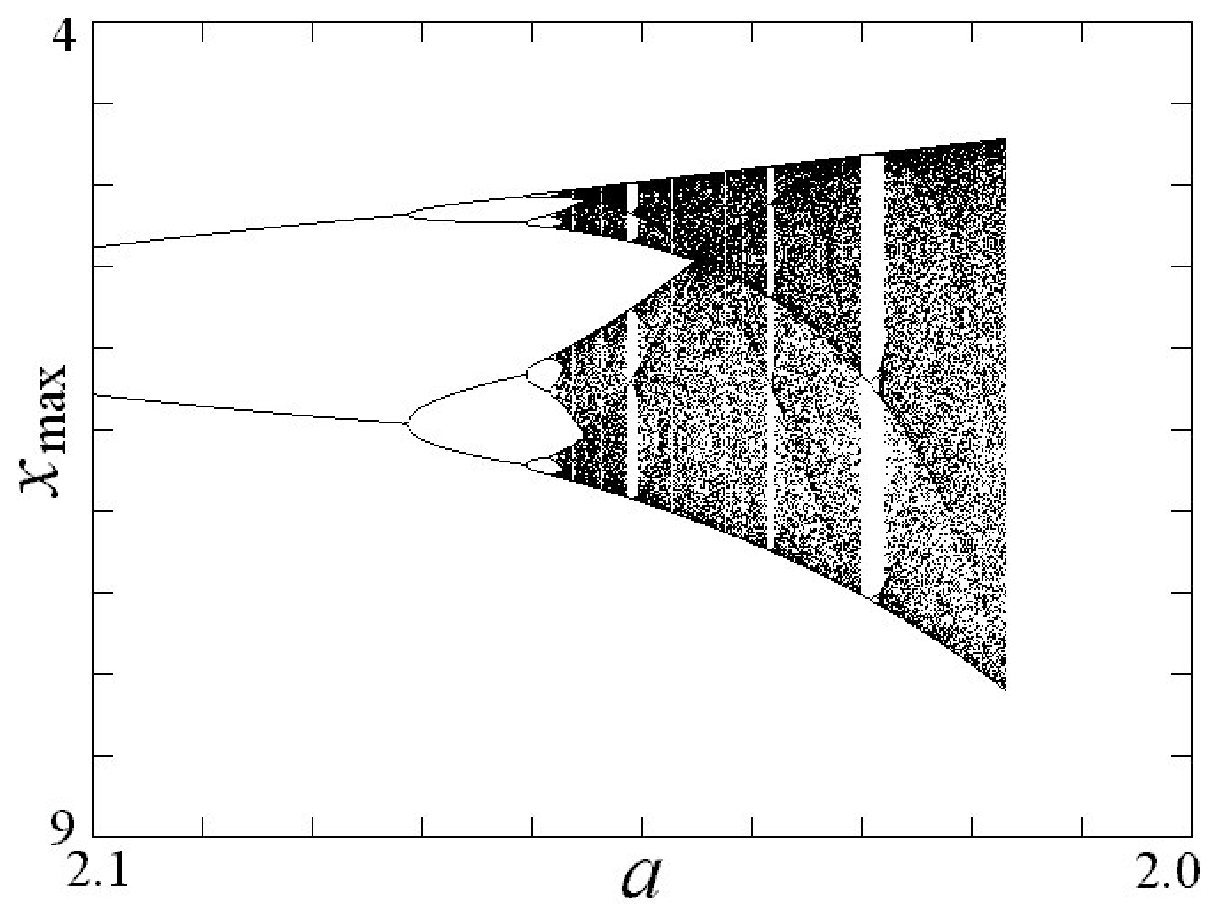
\includegraphics[width=8.4cm]{bifurcation.eps}    % The printed column width is 8.4 cm.
\caption{Bifurcação: Máximos locais de $x$ com o amortecimento $a$ decrescendo.} 
\label{fig:bifurcation}
\end{center}
\end{figure}

Figuras devem ser centralizadas, e ter uma legenda abaixo. 
% Figures must be centered, and have a caption at the bottom. 

\subsection{Tabelas}

Tabelas devem ser centralizadas, ter uma legenda acima e ser numeradas em arábicos.
Veja a Tabela~\ref{tb:margins} para um exemplo. 

%Tables must be centered and have a caption above them, numbered with
%Arabic numerals. See table~\ref{tb:margins} for an example.

\begin{table}[hb]
\begin{center}
\caption{Margens.}\label{tb:margins}
\begin{tabular}{cccc}
Página & Topo & Baixo & Esquerda/Direita \\\hline
Primeira & 3,5 & 2,5 & 1,5 \\
Demais & 2,5 & 2,5 & 1,5 \\ \hline
\end{tabular}
\end{center}
\end{table}

\subsection{Estágio Final}

Espera-se que os autores respeitem as margens diligentemente. 
Os artigos precisam receber o logo com a data do evento e numeração para
posterior inclusão nos Anais. Se o seu manuscrito viola as margens, você será
chamado a preparar uma nova versão (podendo atrasar a preparação dos Anais), ou 
poderá mesmo ser excluído dos Anais. 

%Authors are expected to mind the margins diligently.  Papers need to
%be stamped with event data and paginated for inclusion in the
%proceedings. If your manuscript bleeds into margins, you will be
%required to resubmit and delay the proceedings preparation in the
%process.

\subsubsection{Margens nas páginas.} Veja a Tabela~\ref{tb:margins} 
para as especificações de margem. Todas as dimensões são em 
\emph{centímetros}.


\subsection{Criação do PDF}

Todas as fontes devem estar incluídas no arquivo PDF. Use uma das seguintes
ferramentas para produzir um PDF de boa qualidade: 
%All fonts must be embedded/subsetted in the PDF file. Use one of the
%following tools to produce a good quality PDF file:

\subsubsection{PDFLaTeX} 
é uma versão especial do \LaTeX, de Han The
Thanh, que produz o PDF diretamente do arquivo \texttt{tex} usando fontes do Tipo-1,
sem passar pelo arquivo \texttt{dvi} padrão. Aceita figuras nos formatos JPEG, PNG e PDF,
mas não PostScript. Figuras produzidas em PostScript encapsulado (EPS) podem
ser convertidas em PDF, por exemplo, com a ferramenta \texttt{epstopdf} ou
com o Adobe Acrobat
Distiller.


%is a special version of LaTeX by Han The
%Thanh which produces PDF output directly using Type-1 fonts instead of
%the standard \texttt{dvi} file. It accepts figures in JPEG, PNG, and PDF
%formats, but not PostScript. Encapsulated PostScript figures can be
%converted to PDF with the \texttt{epstopdf} tool or with Adobe Acrobat
%Distiller.

\subsubsection{Gerar o PDF a partir do PostScript} 
é a meneira clássica de produzir arquivos PDF do \LaTeX. Os passos são: 

%is the classical way of
%producing PDF files from LaTeX. The steps are:

\begin{enumerate}
  \item Produza um arquivo \texttt{dvi} rodando \texttt{latex} duas vezes. 
%  Produce a \texttt{dvi} file by running \texttt{latex} twice.
  \item Produza um arquivo PostScript (\texttt{ps}) com \texttt{dvips}.
  %  Produce a PostScript (\texttt{ps}) file with \texttt{dvips}.
  \item Produza um arquivo PDF com \texttt{ps2pdf} ou Adobe Acrobat
  Distiller.
%  Produce a PDF file with \texttt{ps2pdf} or Adobe Acrobat
%  Distiller.
\end{enumerate}

\subsection{Copyright}

A SBA ou os organizadores do congresso devem requerer, no momento devido, 
um formulário de transferência de {\em Copyright}. Mais informações serão
dadas no {\em site} do congresso.
%IFAC will put in place an electronic copyright transfer system in due
%course. Please \emph{do not} send copyright forms by mail or fax. More
%information on this will be made available on IFAC website.


\section{Unidades}

Use preferencialmente unidades do Sistema Internacional (SI). Outras unidades
podem ser utilizadas como unidades secundárias (entre parênteses). Isto se aplica
em armazenamento de dados. Escreva,
por exemplo,  ``$15\,\mathrm{Gb}/\mathrm{cm}^2$ ($100\,\mathrm{Gb}/\mathrm{in}^2$)''. 
Uma exceção é quando unidades inglesas são usadas na identificação de algum item
comercial, como ``disco de 3.5 polegadas''. Evite misturar unidades SI com outras, 
como por exemplo corrente elétrica em amperes e campo magnético em oersteds. 
Isso frequentemente causa confusão, pois as equações não batem dimensionalmente. 
Se você realmente precisar usar unidades mistas, deixe claro as unidades para cada
termo em uma equação. A unidade SI para força do campo magnético 
$\mathbf{H}$ é $\mathrm{A}/\mathrm{m}$. No entanto, se você quiser utilizar unidades
de  $\mathrm{T}$, 
refira-se à densidade de fluxo magnético $\mathbf{B}$ ou
força do campo magnético simbolizada por $\mu_0\,\mathbf{H}$. 
Use um ponto centralizado para separar unidades compostas, p. ex.,  
``$\mathrm{A} \cdot \mathrm{m}^2$''.

%Use SI as primary units. Other units may be used as secondary units
%(in parentheses). This applies to papers in data storage. For example,
%write ``$15\,\mathrm{Gb}/\mathrm{cm}^2$ ($100\,\mathrm{Gb}/\mathrm{in}^2$)''. 
%An exception is when
%English units are used as identifiers in trade, such as ``3.5 in
%disk drive''. Avoid combining SI and other units, such as current in
%amperes and magnetic field in oersteds. This often leads to confusion
%because equations do not balance dimensionally. If you must use mixed
%units, clearly state the units for each quantity in an equation.  The
%SI unit for magnetic field strength $\mathbf{H}$ is $\mathrm{A}/\mathrm{m}$. However, if you wish to
%use units of $\mathrm{T}$, either refer to magnetic flux density $\mathbf{B}$ or
%magnetic field strength symbolized as $\mu_0\,\mathbf{H}$. Use the center dot to
%separate compound units, e.g., ``$\mathrm{A} \cdot \mathrm{m}^2$''.

\section{Dicas Úteis}

\subsection{Figuras e Tabelas}

Legendas dos eixos das figuras são frequentemente uma fonte de confusões. Use
palavras ao invés de símbolos. Por exemplo, escreva a quantidade ``Magnetização'',
ou ``Magnetização M'', não apenas ``M''. Coloque unidades entre parênteses. Não marque
os eixos apenas com unidades ou quantidades. Por exemplo, escreva 
``Temperatura ($\mathrm{K}$)'', não ``$\mbox{Temperature}/\mathrm{K}$''.

Multiplicandos podem ser especialmente confusos. Escreva  ``Magnetização 
($\mathrm{kA}/\mathrm{m}$)'' ou ``Magnetização ($10^3 \mathrm{A}/\mathrm{m}$)''. 
Não escreva 
``Magnetização $(\mathrm{A}/\mathrm{m}) \times 1000$'' pois o leitor não saberá
se a legenda do eixo significa 
$16000\,\mathrm{A}/\mathrm{m}$ ou $0.016\,\mathrm{A}/\mathrm{m}$.

%Figure axis labels are often a source of confusion. Use words rather
%than symbols. As an example, write the quantity ``Magnetization'', or
%``Magnetization M'', not just ``M''. Put units in parentheses. Do not
%label axes only with units.  For example, write ``Magnetization
%($\mathrm{A}/\mathrm{m}$)'' or ``Magnetization ($\mathrm{A} \mathrm{m}^{-1}$)'', not just
% ``$\mathrm{A}/\mathrm{m}$''. Do not
%label axes with a ratio of quantities and units. For example, write
%``Temperature ($\mathrm{K}$)'', not ``$\mbox{Temperature}/\mathrm{K}$''.
%
%Multipliers can be especially confusing. Write ``Magnetization
%($\mathrm{kA}/\mathrm{m}$)'' or ``Magnetization ($10^3 \mathrm{A}/\mathrm{m}$)''. Do not write
%``Magnetization $(\mathrm{A}/\mathrm{m}) \times 1000$'' because the reader would not know
%whether the axis label means $16000\,\mathrm{A}/\mathrm{m}$ or $0.016\,\mathrm{A}/\mathrm{m}$.

\subsection{Referências}

Use referências no estilo Harvard (veja no final deste documento). Com
\LaTeX, você pode processar uma base externa de dados bibliográficos 
usando \texttt{bibtex},\footnote{Nesse caso, você também vai precisar do arquivo \texttt{ifacconf.bst}, que é parte do pacote \texttt{ifacconf\_latex.zip}} ou então inserir
as referências diretamente na seção correspondente. Evite as notas de rodapé.
Por favor, note que o estilo preferido de referências é o que se encontra no
final deste documento. Artigos que não foram publicados devem ser citados 
como ``unpublished''. Use maiúscula apenas na primeira palavra do título
do artigo, exceto para nomes próprios, acrônimos e símbolos. Todos os autores
devem ser explicitados nos artigos. Note que você pode citar com \texttt{\textbackslash cite\{label\}} quando a citação fizer parte do texto ou com \texttt{\textbackslash citep\{label\}}.

%Use Harvard style references (see at the end of this document). With
%\LaTeX, you can process an external bibliography database 
%using \texttt{bibtex},\footnote{In this case you will also need the \texttt{ifacconf.bst}
%file, which is part of the \texttt{ifaconf} package.}
%or insert it directly into the reference section. Footnotes should be avoided as
%far as possible.  Please note that the references at the end of this
%document are in the preferred referencing style. Papers that have not
%been published should be cited as ``unpublished''.  Capitalize only the
%first word in a paper title, except for proper nouns and element
%symbols.

\subsection{Abreviações e Acrônimos}

Defina as abreviações e os acrônimos na primeira ocorrência do texto do artigo, 
mesmo se foram definidos no abstract. Abreviações conhecidas, como SI ou SBA, não
precisam ser definidas. Abreviações que incorporam pontos não devem conter espaços
(escreva ``C.N.R.S.'', não ``C. N. R. S.''). Não use abreviações no título, exceto
se forem inevitáveis. 
%Define abbreviations and acronyms the first time they are used in the
%text, even after they have already been defined in the
%abstract. Abbreviations such as IFAC, SI, ac, and dc do not have to be
%defined. Abbreviations that incorporate periods should not have
%spaces: write ``C.N.R.S.'', not ``C. N. R. S.'' Do not use abbreviations
%in the title unless they are unavoidable (for example, ``IFAC'' in the
%title of this article).

\subsection{Equações}

Numere as equações de forma consecutiva, com números entre parênteses
encostados no lado direito da
margem, como em~\eqref{eq:sample}. Para tornar suas equações mais compactas,
você pode usar $/$, a função $\exp$, ou expoentes apropriados. Use parênteses para
evitar ambiguidades. Pontue as equações quando estas forem parte do texto, como em
%Number equations consecutively with equation numbers in parentheses
%flush with the right margin, as in (\ref{eq:sample}).  To make your equations more
%compact, you may use the solidus ($/$), the $\exp$ function, or
%appropriate exponents. Use parentheses to avoid ambiguities in
%denominators. Punctuate equations when they are part of a sentence, as
%in

\begin{multline} 
\int_0^{r_2}  F (r, \varphi ) dr d\varphi =  [\sigma r_2 / (2 \mu_0 )] \\
\times   \int_0^{\infty} \exp(-\lambda |z_j - z_i |) \lambda^{-1} J_1 (\lambda  r_2 ) J_0 (\lambda r_i ) d\lambda 
\label{eq:sample2}
\end{multline}

Certifique-se que os símbolos em sua equação tenham sido previamente definidos (ou defina-se imediatamente depois). Símbolos devem aparecer em itálico ($T$ pode
se referir à temperatura, mas T é a unidade tesla). 
Refira-se a ``(\ref{eq:sample})'', não ``Eq. (\ref{eq:sample})'' ou ``equação
(\ref{eq:sample})'', exceto no começo de uma frase: ``Equação~(\ref{eq:sample}) é \ldots''. 
%might refer to temperature, but T is the unit tesla). 
%Be sure that the symbols in your equation have been defined before the
%equation appears or immediately following. Italicize symbols ($T$
%might refer to temperature, but T is the unit tesla). Refer to
%``(\ref{eq:sample})'', not ``Eq. (\ref{eq:sample})'' or ``equation
%(\ref{eq:sample})'', except at the beginning of a sentence: ``Equation
%(\ref{eq:sample}) is \ldots''.

\subsection{Outras Recomendações}

Deixe um espaço após pontos e vírgulas. 
Uma afirmação entre parênteses no final de uma sentença é pontuada exteriormente
(assim). (Uma frase entre parênteses é pontuada internamente.) Evite contrações
(por exemplo, ``prá'' chegar ao resultado --- use ``para''). 




\section{Conclusão}

Uma seção com a conclusão não é obrigatória. Apesar de uma conclusão poder ser usada
para rever os principais pontos do artigo, não de deve simplesmente replicar o resumo
na conclusão. Uma conclusão pode ser utilizada para frisar a importância do artigo
ou delinear extensões e aplicações. 


\section*{Agradecimentos}
Coloque aqui seus agradecimentos. 

\bibliography{ifacconf}             % bib file to produce the bibliography
                                                     % with bibtex (preferred)
                                                   
%\begin{thebibliography}{xx}  % you can also add the bibliography by hand

%\bibitem[Able(1956)]{Abl:56}
%B.C. Able.
%\newblock Nucleic acid content of microscope.
%\newblock \emph{Nature}, 135:\penalty0 7--9, 1956.

%\bibitem[Able et~al.(1954)Able, Tagg, and Rush]{AbTaRu:54}
%B.C. Able, R.A. Tagg, and M.~Rush.
%\newblock Enzyme-catalyzed cellular transanimations.
%\newblock In A.F. Round, editor, \emph{Advances in Enzymology}, volume~2, pages
%  125--247. Academic Press, New York, 3rd edition, 1954.

%\bibitem[Keohane(1958)]{Keo:58}
%R.~Keohane.
%\newblock \emph{Power and Interdependence: World Politics in Transitions}.
%\newblock Little, Brown \& Co., Boston, 1958.

%\bibitem[Powers(1985)]{Pow:85}
%T.~Powers.
%\newblock Is there a way out?
%\newblock \emph{Harpers}, pages 35--47, June 1985.

%\bibitem[Soukhanov(1992)]{Heritage:92}
%A.~H. Soukhanov, editor.
%\newblock \emph{{The American Heritage. Dictionary of the American Language}}.
%\newblock Houghton Mifflin Company, 1992.

%\end{thebibliography}

\appendix
\section{Sumário da gramática sânscrita}    % Each appendix must have a short title.
\section{Algum vocabulário maia}              % Sections and subsections are supported  
                                                                         % in the appendices.
\end{document}
